% !TeX root = ../../thesis.tex

\subsection{Test Suite Assessment}

\subsubsection{Coverage}
\noindent The most frequently used metric to measure the quantity and thoroughness of a test suite is the \emph{code coverage} or \emph{test coverage} \cite[p.~467]{8016712}. The test coverage is expressed as a percentage and indicates which fraction of the application code is affected by code in the test suite. Internally, this works by augmenting every statement in the application code using binary instrumentation. A hook is inserted before and after every statement to keep track of which statements are executed during tests. Many different criteria exist to interpret these instrumentation results and thus to express the fraction of covered code \cite{Myers:2011:AST:2161638}, the most commonly used ones are \emph{statement coverage} and \emph{branch coverage}.

\paragraph*{Statement coverage} expresses the fraction of code statements that are executed in any test of the test suite \cite{6588537}, out of all executable statements in the application code. Analogously, the fraction of lines covered by a test may be used to calculate the \emph{line coverage} percentage. Since one statement can span multiple lines and one line may also contain more than one statement, both of these criteria implicitly represent the same value. Statement coverage is heavily criticised in literature \cite[p.~37]{Myers:2011:AST:2161638}, since it is possible to achieve a statement coverage percentage of 100\% on a code fragment which can be proven to be incorrect. Consider the code fragment in \autoref{lst:statement-coverage-fail}. If a test would call the \texttt{example}-function with arguments $\{a = 1, b = 2\}$, the test will pass and every statement will be covered, resulting in a statement coverage of 100\%. However, it is clear to see that if the function would be called with arguments $\{a = 0, b = 0\}$, a \emph{division-by-zero} error would be raised, resulting in a crash. This very short example already indicates that statement coverage is not trustworthy, yet it may still be useful for other purposes, such as detecting unreachable code which may safely be removed.

\begin{listing}
	\begin{lstlisting}[language=C]
		int example(int a, int b) {
			if (a == 0 || b != 0) {
				return a / b;
			}
		}
	\end{lstlisting}
	\captionsetup{skip=-2pt}
	\caption{Example of irrelevant statement coverage in C.}
	\label{lst:statement-coverage-fail}
\end{listing}

\paragraph*{Branch coverage} on the other hand, requires that every branch of a conditional statement is traversed at least once \cite[p.~37]{Myers:2011:AST:2161638}. For an \texttt{if}-statement, this results in two tests being required, one for every possible outcome of the condition (\texttt{true} or \texttt{false}). For a \texttt{loop}-statement, this requires a test case in which the loop body is never executed and another test case in which the loop body is always executed. Remark that while this criterion is stronger than statement coverage, it is still not sufficiently strong to detect the bug in \autoref{lst:statement-coverage-fail}. In order to mitigate this, \emph{multiple-condition coverage} \cite[p.~40]{Myers:2011:AST:2161638} is used. This criterion requires that for every conditional statement, every possible combination of subexpressions is evaluated at least once. Applied to \autoref{lst:statement-coverage-fail}, the \texttt{if}-statement is only covered if the following four cases are tested, which is sufficient to detect the bug.
\begin{itemize}
	\item $a = 0, b = 0$
	\item $a = 0, b \neq 0$
	\item $a \neq 0, b = 0$
	\item $a \neq 0, b \neq 0$
\end{itemize}

\noindent It should be self-evident that achieving and maintaining a coverage percentage of 100\% at all times is critical. However, this does not necessarily imply that all lines, statements or branches need to be covered explicitly \cite{dein_2019}. Some parts of the code might simply be irrelevant or untestable. Examples include wrapper or delegation methods that simply call a library function. All major programming languages have frameworks and libraries available to collect coverage information during test execution, and each of these frameworks allows the developer to exclude parts of the code from the final coverage calculation. As of today, the most popular options are JaCoCo\footnote{\url{https://www.jacoco.org/jacoco/}} for Java, coverage.py\footnote{\url{https://github.com/nedbat/coveragepy}} for Python and simplecov\footnote{\url{https://github.com/colszowka/simplecov}} for Ruby. These frameworks are able to generate in-depth statistics on which parts of the code are covered and which parts require more tests, as illustrated in \autoref{fig:coverage-statistics}.

\subsubsection{Mutation testing}
Whereas code coverage can be used to identify whether or not a part of the code is currently affected by the test suite, \emph{mutation testing} can be used to measure its quality and ability to detect future failures. This technique creates several syntactically different instances of the source code, referred to as \emph{mutants}. A mutant can be created by applying one or more \emph{mutation operators} to the original source code. These mutation operators are aimed at simulating typical mistakes that developers tend to make, such as the introduction of off-by-one errors, removal of statements and replacement of logical connectors \cite{Offutt2001}. The \emph{mutation order} refers to the amount of mutation operators that have been applied consecutively to an instance of the code. This order is traditionally rather low, as a result of the \emph{Competent Programmer Hypothesis}, which states that programmers develop programs which are near-correct \cite{5487526}.

\paragraph*{Creating and evaluating} the mutant versions of the code is a computationally expensive process, which is why very few software developers have employed this technique in practice. This process is very straightforward, as illustrated in \autoref{fig:mutation-testing}. First of all, the mutation system takes the original program $P$ and a set of test cases $T$. Then, several mutation operators are applied to construct a large set of mutants $P'$. The next step is to evaluate every test case $t$ on the original program $P$ to verify its correctness, this is a task that needs to be performed manually. If at least one of these test cases proves incorrect, a bug has been found in the original program, which needs to be resolved before the mutation analysis can continue. When $P$ successfully passes every test case, every test case are evaluated for each of the mutants. A mutant $p'$ is said to be ``killed'' if its output is different from $P$ for at least one test case, otherwise it is considered ``surviving''. After executing all test cases, the set of surviving mutants should be analysed in order to introduce subsequent test cases that can be used to kill them. However, it is also possible that the surviving mutants are functionally equivalent to $P$. This is a problem that cannot be decided automatically, since the detection of program equivalence is impossible \cite{5487526, Offutt2001}.

\begin{figure}[htbp!]
	\centering
	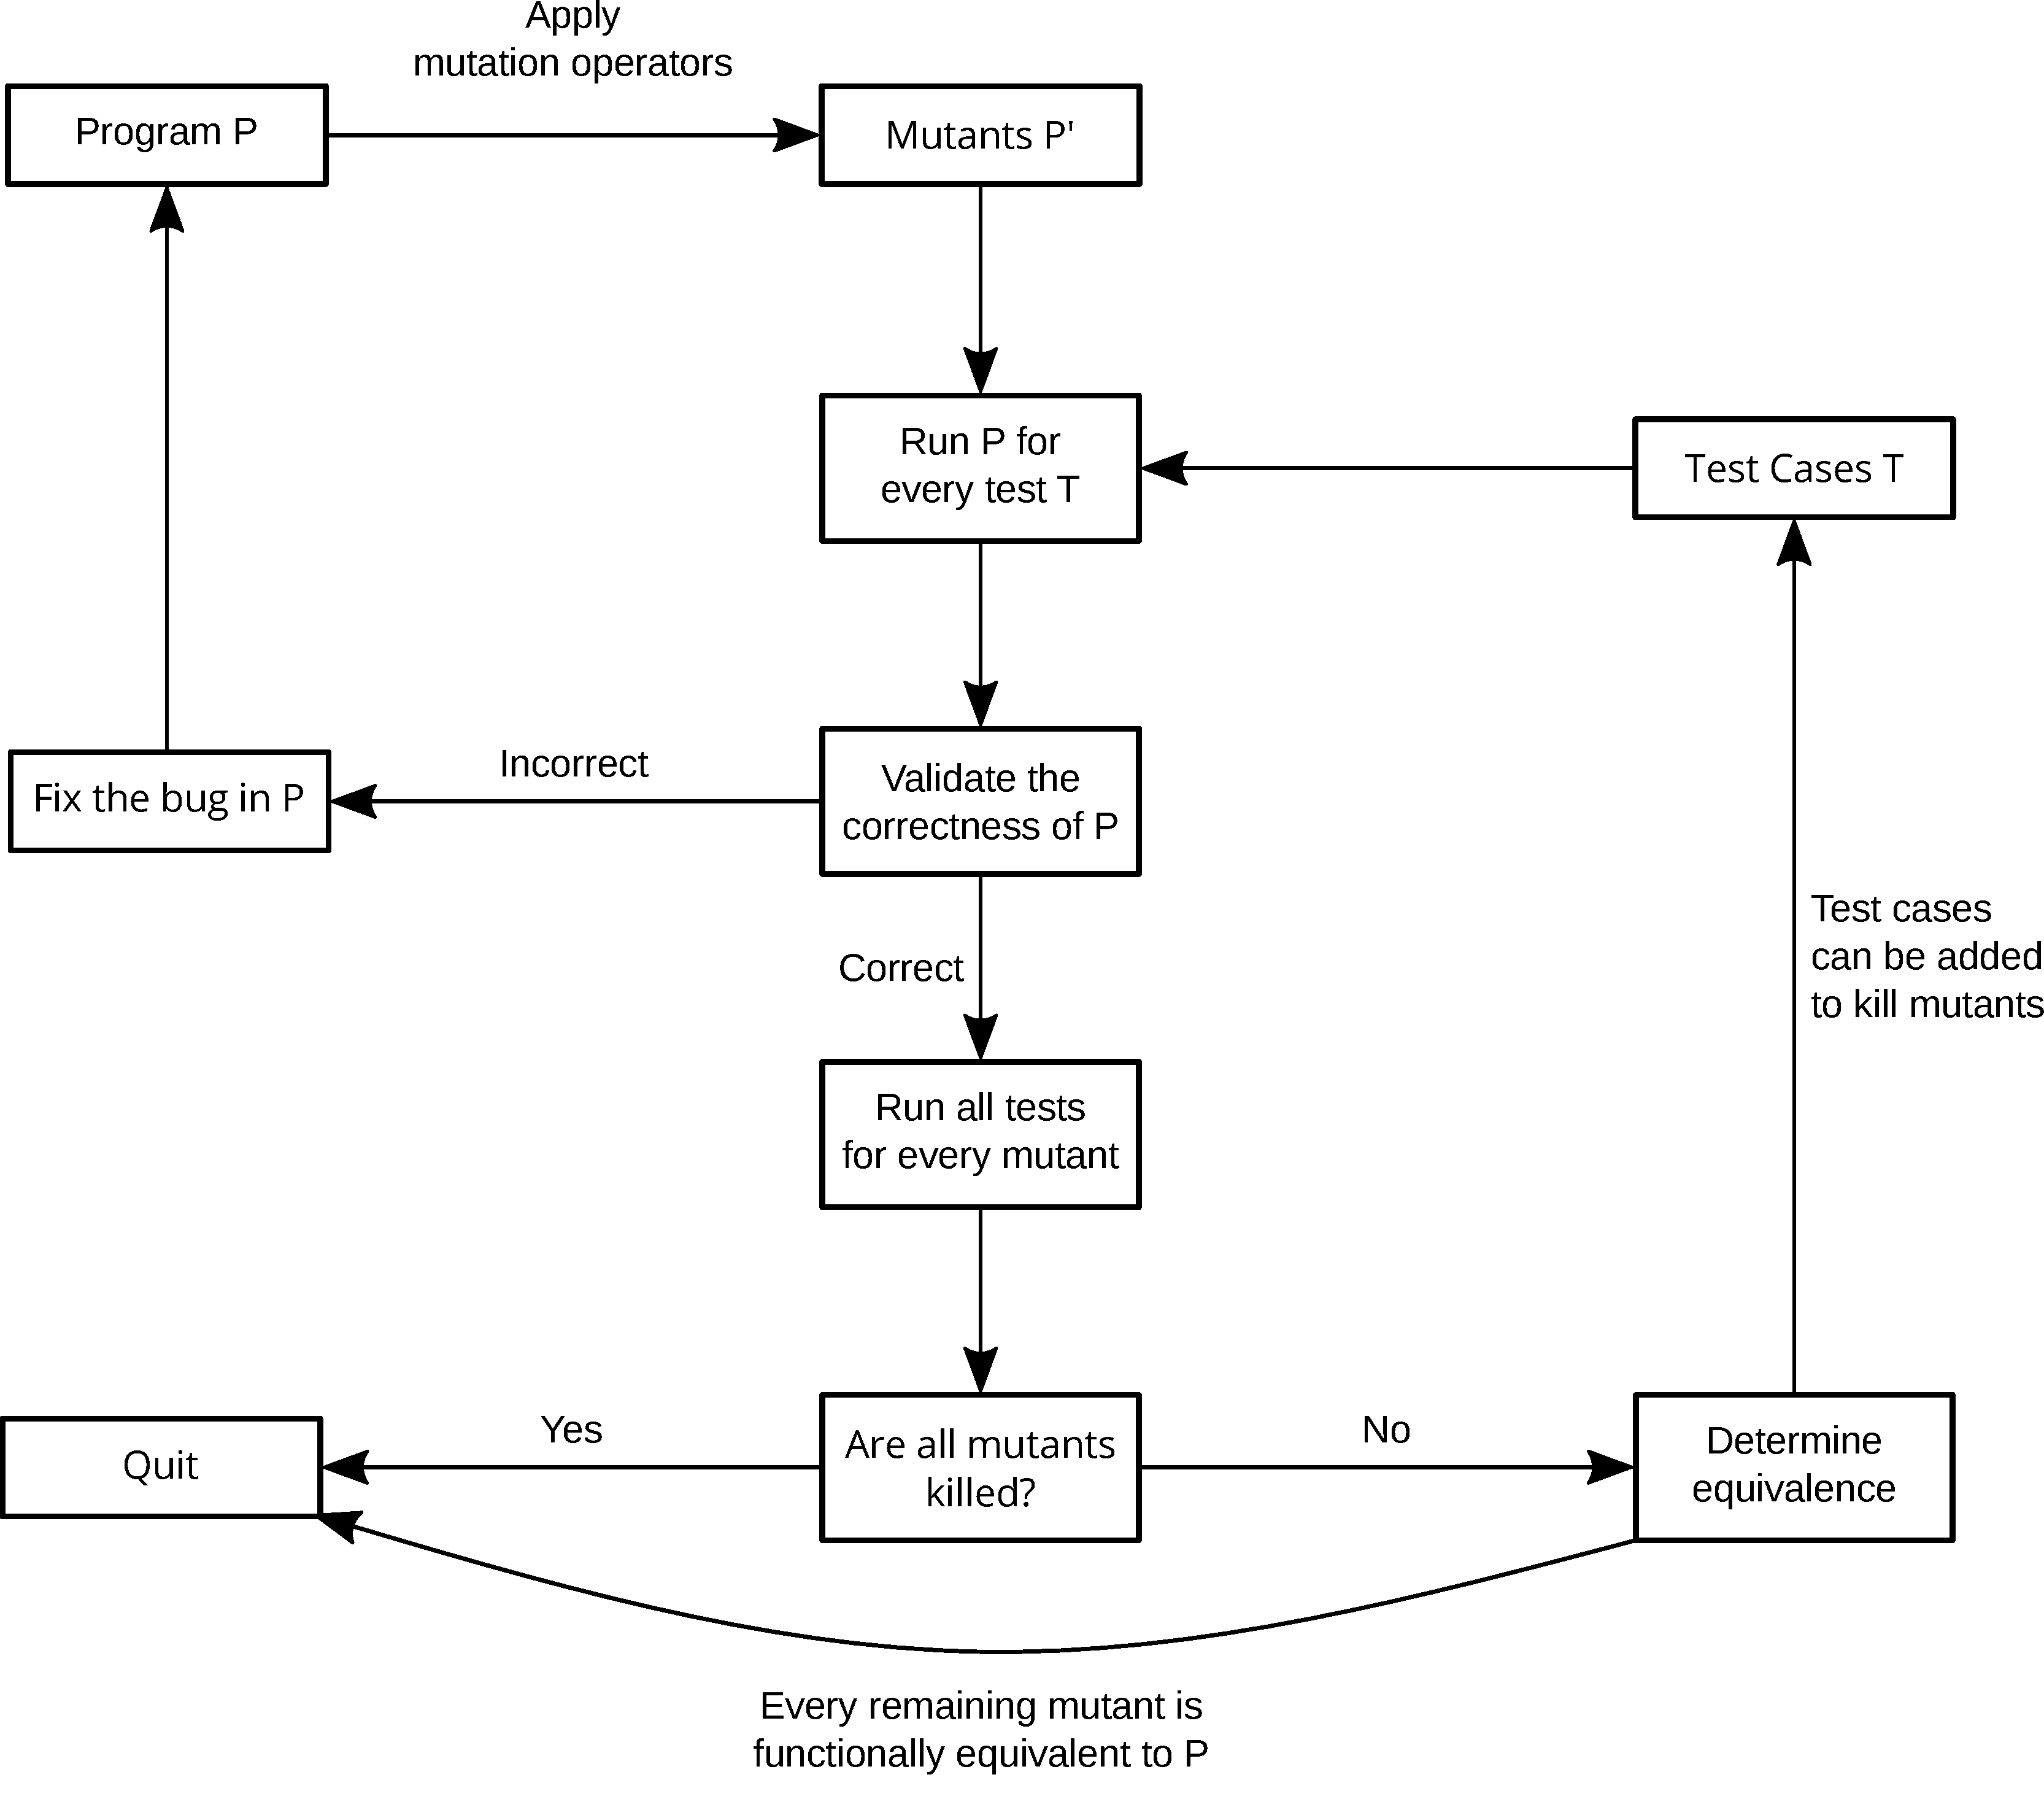
\includegraphics[width=\textwidth]{assets/mutation-testing.pdf}
	\caption{Process of Mutation Testing (based on \cite{Offutt2001})}
	\label{fig:mutation-testing}
\end{figure}

\noindent After every mutant has either been killed or marked equivalent to the original problem, a \emph{mutation score} is calculated using \autoref{eq:mutant-score}. In a perfect test suite, this score should be equal to 1, indicating that the test suite was able to detect every mutant. 

\begin{equation}\label{eq:mutant-score}
	\text{Mutant Score} = \frac{\text{killed mutants}}{\text{non-equivalent mutants}}
\end{equation}


\begin{figure}[htbp!]
	\centering
	\subfloat[JaCoCo coverage report of \url{https://github.com/thepieterdc/dodona-api-java}]{%
		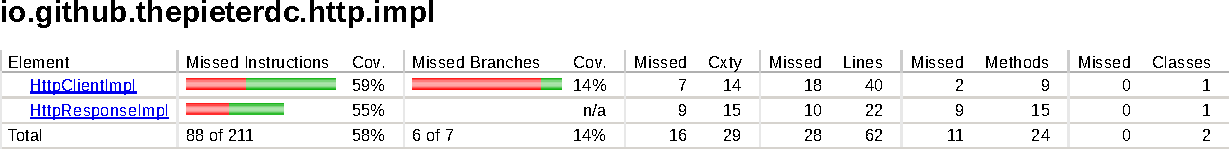
\includegraphics[clip,width=\textwidth]{assets/coverage-jacoco.pdf}
	}
	\newline
	\subfloat[coverage.py report of \url{https://github.com/codecov/example-python}]{%
		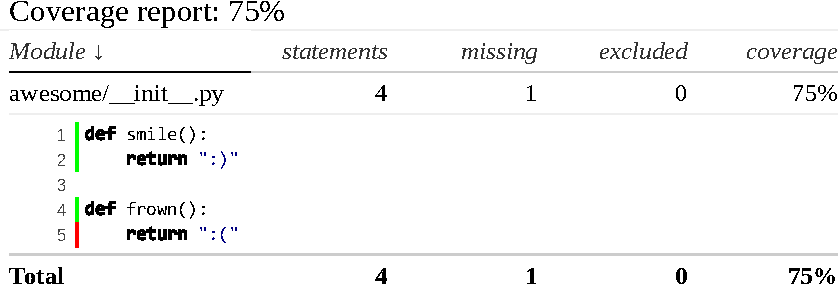
\includegraphics[clip,width=\textwidth]{assets/coverage-coveragepy.pdf}
	}
	\newline
	\subfloat[simplecov report of \url{https://github.com/dodona-edu/dodona}]{%
		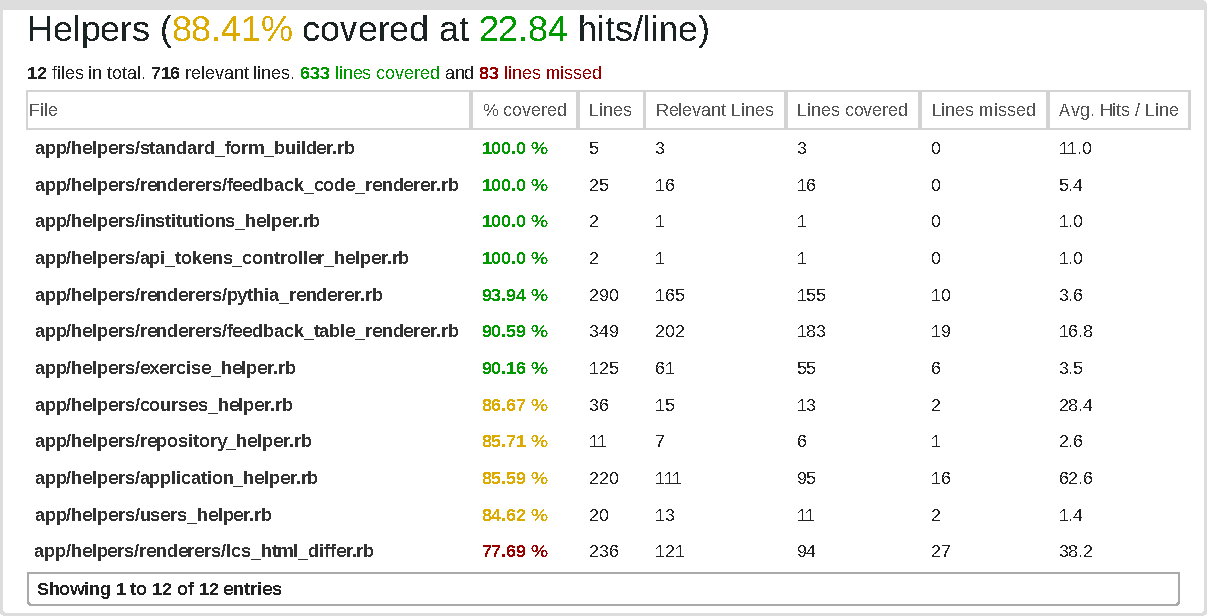
\includegraphics[clip,width=\textwidth]{assets/coverage-simplecov.pdf}
	}
	\caption{Statistics from Code coverage tools}
	\label{fig:coverage-statistics}
\end{figure}